\section{Design and Models}
\label{chapter:design}

In this chapter, we describe the overall design of our disaster monitoring backend system in details.
Firstly, we propose our system architecture of this disaster monitoring;
Then we specify and justify our most critical system components such as databases design, 
\textbf{Player Task Generator (PTG)\label{idx:ptg}}, \textbf{Player Rating Model (PRM)\label{idx:prm}} 
as well as \textbf{Disaster Evaluation Model (DEM)\label{idx:dem}}.

With these components, model and databases, the disaster monitoring system can handle
common problems in human computation system, such as cold start, malicious player detection, etc. 
It is also expandable, portable and can be easily applied to any other same image selection 
and tagging based human computation system in different areas.

\subsection{System Architectures}

Figure \ref{fig:arch} illustrate the overall disaster system design.
The system databases are composed of two different type of databases. 
The first database \textbf{PlayerDB} combines \textbf{TrustedDB} and \textbf{UntrustedDB} 
where persistent the player property and raw tagging inputs whether the overall result is reliable or not.
The second database is called \textbf{ResultDB} where persistent the reliable player inputs.

\begin{figure}[htp]
\centering
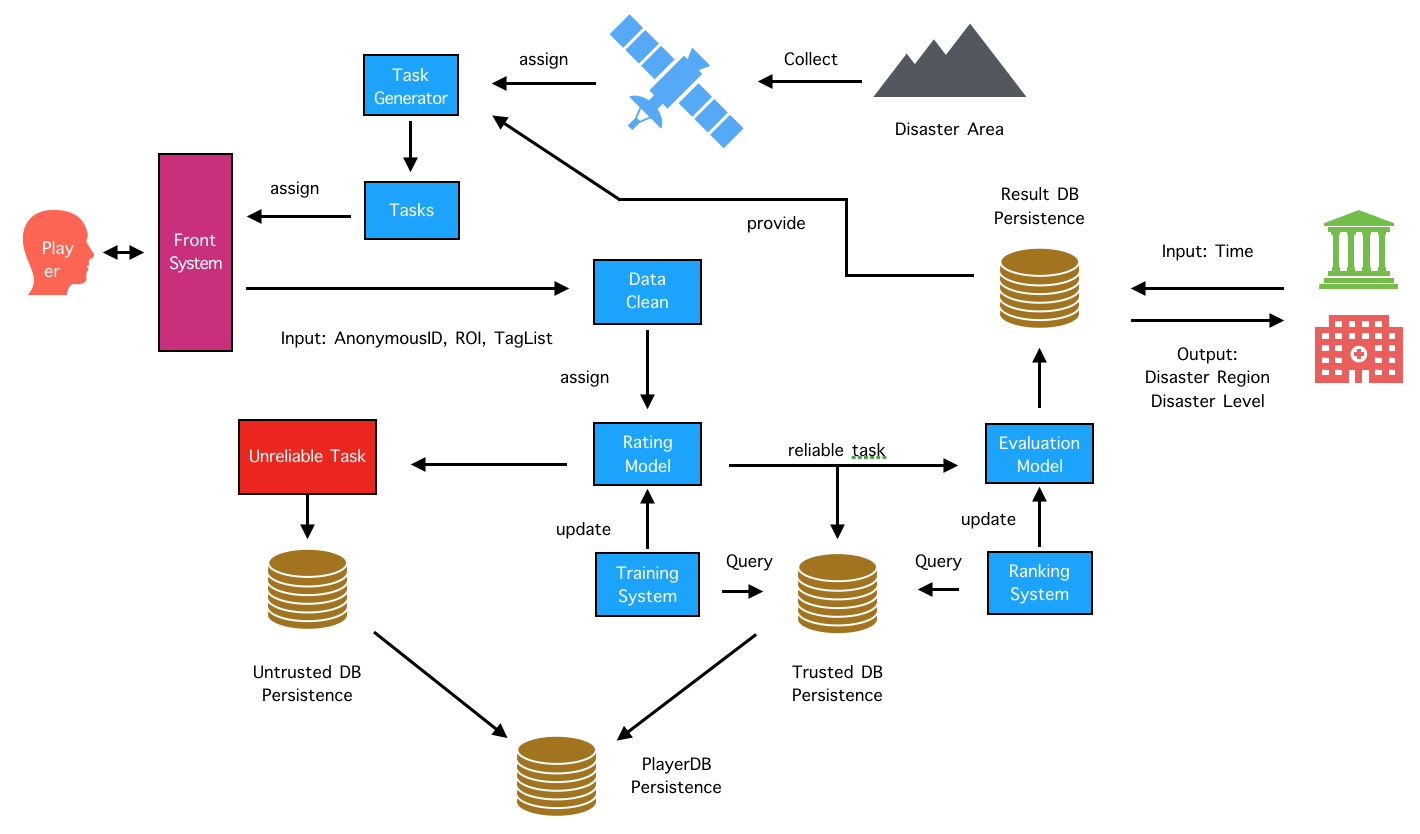
\includegraphics[width=0.9\textwidth]{figures/system2}
\caption{System Design Overview}
\label{fig:arch}
\end{figure}

For this architecture design, one can simplify the overall data flow into tree main steps 
that describes as follows:

\begin{itemize}

\item [Step 1.]  Player task generating: 
We propose the \textbf{\hyperref[idx:ptg]{PTG}}
that combines trusted results from TrustedDB, 
and separate new images from satellite, then assign this binding to the future players.

\item [Step 2.] Malicious player detection: 
A reliable player shall pass the malicious detection algorithm (describe in algorithm \ref{algo:malicious})
inside the \textbf{\hyperref[idx:prm]{PRM}}. 
Once the player is not a malicious player, then system will mark all the results from this player
as a reliable result and then send it into next step.

\item [Step 3.] Evaluating disaster level:  the system reuse the reliable player inputs 
into \textbf{\hyperref[idx:dem]{DEM}} and calculate the disaster level of the monitoring region
 as well as persistent it in the second database ResultDB.

\end{itemize}

After these three main steps, stakeholders are able to retrieve monitoring results from
the database ResultDB. 

\subsection{System Components}

\subsubsection{Database Fields}

We describe the system database PlayerDB 
fields as well as the fields of database ResultDB first in listing \ref{lst:playerdb}
and \ref{lst:resultdb}.

In this disaster monitoring system, our participants \textbf{do not need to register accounts},
and the system backend shall \textbf{generate and assign an} \emph{player\_id} \textbf{to each player} according to 
the user scenario (such as IP address, network status, system information et cetera).
This function significantly accelerate player to participate in this game. 
Thus, the \textbf{PlayerDB} stores the \emph{player\_id} to detect the same players if they participate next time. 
The player will accomplish different game tasks; each task result shall store in the tasks filed.

\noindent\begin{minipage}{.45\textwidth}
\begin{lstlisting}[
    caption={Example of PlayerDB Data},
    label={lst:playerdb}
]
[
 {
  "player_id": "E3A6F124-4A6C-4C6E-B7F1-F8BC9A7381CC",
  "tasks": [
   {
    "image_id": "3A21E99E-F074-454B-A590-8D8C5ABD8E77",
    "image_at": "2017-07-31 11:28:40",
    "reliable": true,
    "ROIs": [
     {
      "x": 103, "y": 121,
      "height": 56,
      "width": 78,
      "tags": ["burning building", "explosion"]
     }
    ]
   }
  ]
 }
]
\end{lstlisting}
\end{minipage}\hfill
\begin{minipage}{.45\textwidth}
\begin{lstlisting}[
  caption={Example of ResultsDB Data},
  label={lst:resultdb}
]
[
 {
  "region_id": "FBEB6204-0B94-4811-94F0-9DDC5FBBE6D8",
  "history": [
   {
    "image_id": "3A21E99E-F074-454B-A590-8D8C5ABD8E77",
    "image_at": "2017-07-31 11:28:40",
    "ROIs": [
     {
      "x": 103, "y": 121,
      "height": 56,
      "width": 78,
      "tags": ["burning building", "explosion"]
     }
    ]
   }
  ]
 }
]
\end{lstlisting}
\end{minipage}

In the \textbf{ResultDB}, a \emph{region\_id} is unique and assigned by our system. A region has its
monitoring history and composed by its separate images, the only difference between PlayerDB and ResultDB is
ResultDB only stores reliable data (no \emph{reliable} field) and images organized by its related region.

To explain other fields and establish our models, we describe few basic definitions for the system models first.

\begin{definition}
\label{def:roi}
\emph{The \textbf{Region of Interests (ROI)} is an indicator that represents the one of the selected two dimensional regions from player. 
The $i$-th ROI from player $p$ in image $k$ at image creation time $t$ is denoted by $ROI_{p,i,k,t}$.}
\end{definition}

Considering image $k$ \textbf{implies} its creation time $t$ (an image alwasy has its creation time), for convenience, 
we usually \textbf{simplify $ROI_{p,i,k,t}$ to $ROI_{p,i,k}$}.
For instance, figure \ref{fig:roi} shows few examples of ROI on different images.

\begin{figure}[htp]
\centering
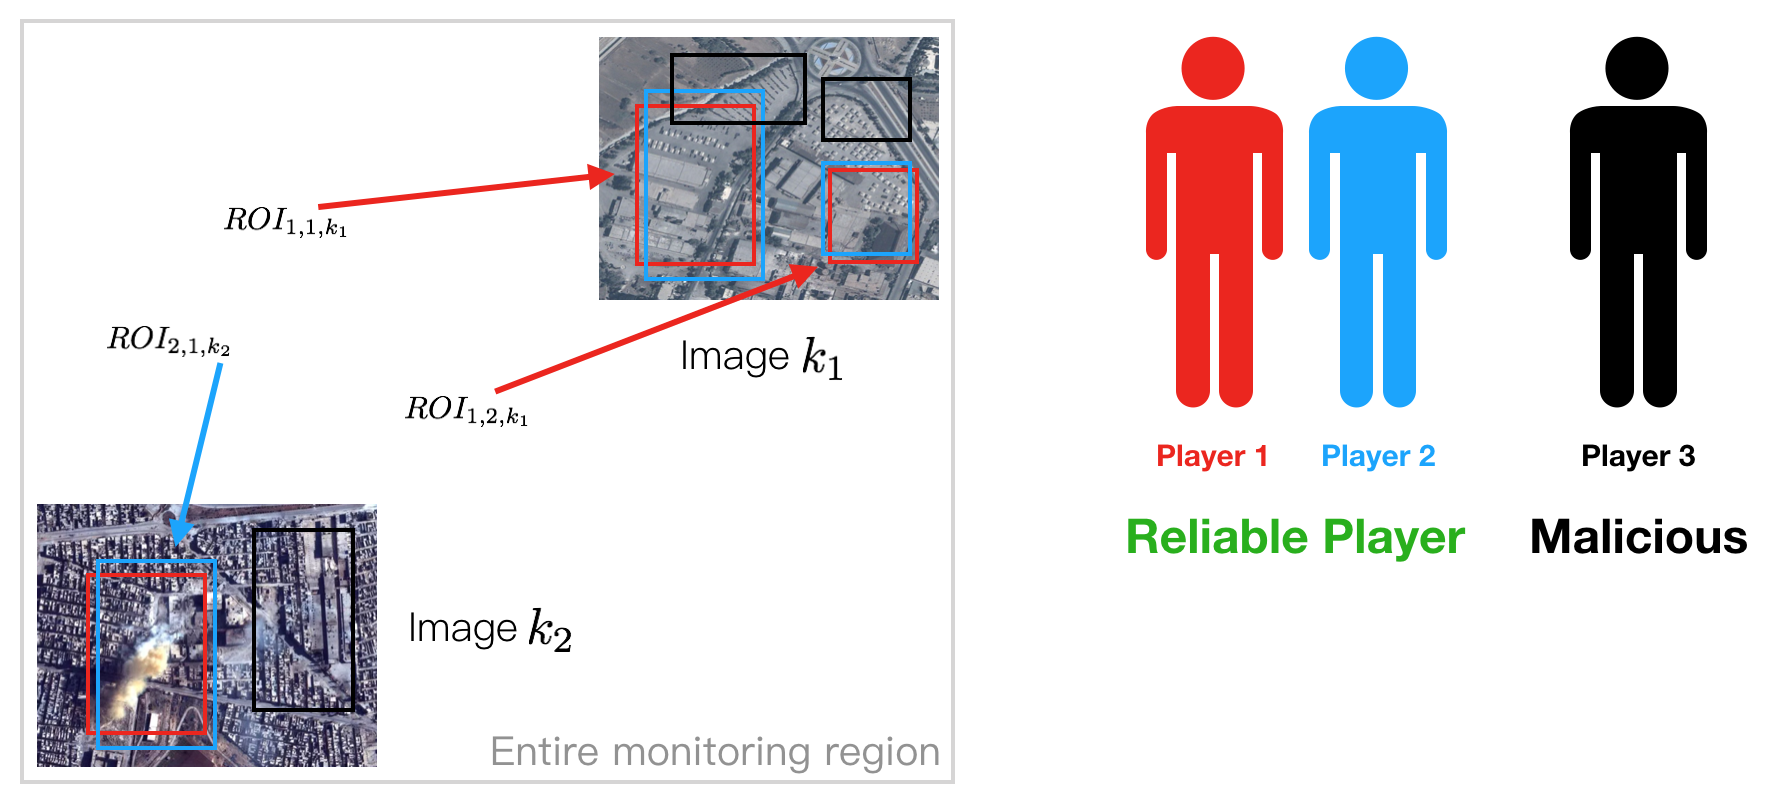
\includegraphics[width=0.9\textwidth]{figures/roi}
\caption{Examples of Region of Interests (ROI)}
\label{fig:roi}
\end{figure}

With this definition, our system players are able to select ROIs for each image as well as capable of select tags for each ROI.
Thus, the \emph{tasks} field in PlayerDB is an array object, stores each player image result with an assigned \emph{image\_id}.
Each object in the \emph{tasks} array has a field \emph{reliable}, which indicates the reliability for this object task;
Each object also contains a \emph{ROIs} field, which is an array object that contains the player inputs for this object image;
Each ROI object in the ROIs field has four properties that describes the ROI geometric location: \emph{x, y, height, width}, and 
also a \emph{tags} array field that describes the input tags for this image from this player.


For \emph{tags} field, game players can select the related tags for each ROI, and stores in this array. 
However, systems like ESP \cite{von2004labeling}, ARTigo \cite{wieser2013artigo} have proved that 
human inputs are valuable and useful. Therefore we allows player input their own tags. That is, 
\textbf{each tag can only selects once, and players allow to input their own new tags for the selected ROIs.} 
Then, We define the ROI tag vector for the model design:

\begin{definition}
\label{def:tagv}
\emph{Assuming the database stores $n$ different tags $\text{tag}_1, \text{tag}_2, ..., \text{tag}_n$ for a certain image $k$,
the \textbf{Tag Vector} $T_{p, i, k}$ of $ROI_{p, i, k}$ (the $i$-th ROI in image $k$ of player $p$) is a vector that 
is donated by the following formula:}
\begin{equation}
  T_{p, i, k} = (|\text{tag}_1|, |\text{tag}_2|, ..., |\text{tag}_n|)
\end{equation}
\emph{where
\begin{itemize}
\item $\text{tag}_i$ is the $i$-th tag;
\item $n$ is the number of tags;
\item $|\text{tag}_i|$ is the count of $\text{tag}_i$ in a player task object.
\end{itemize}}
\end{definition}

Note that due to each tag can only selects once, the components of tag vector is \textbf{either 1 or 0} in reality.
This definition performs a popular data preprocessing technique, which called One-Hot Encoding trick \cite{wu2012foundations, liu2002discretization}.
For instance, for a certain image $k$,
there are 5 different tags $\text{tag}_1, \text{tag}_2, \text{tag}_3, \text{tag}_4, \text{tag}_5$ were inputed
by our game player.
Assuming player $p$ selects the first ROI and inputs tags for $ROI_{p, 1, k}$: 
$\{\text{tag}_1, \text{tag}_2, \text{tag}_3, \text{tag}_4\}$, 
player $q$ selects the first ROI and inputs tags for $ROI_{q, 1, k}$:
$\{\text{tag}_1, \text{tag}_3, \text{tag}_4, \text{tag}_5\}$. 
Then tag vector $T_{p, 1, k}$ of $ROI_{p, 1, k}$ is $(1, 1, 1, 1, 0)$ and tag vector
$T_{q, 1, k}$ of $ROI_{q, 1, k}$ is $(1, 0, 1, 1, 1)$.

\subsubsection{Player Task Generator}

The \textbf{\hyperref[idx:ptg]{PTG}} combines task images from satellite and ResultDB.
A player task contains $2n$ different images in random order, that $n$ images are
the untagged new satellite images and $n$ images are tagged images of ResultDB, which means
\hyperref[idx:ptg]{PTG} contains two generating steps:

\begin{itemize}
\item [Step 1.] \hyperref[idx:ptg]{PTG} shall split a monitoring region into small pieces of images, 
and also assign a unique \textbf{image\_id} for each piece 
(The reason is discussed in section \ref{chapter:ethical} for the leakage of data).

\item [Step 2.] \hyperref[idx:ptg]{PTG} shall retrieve tagged images from ResultDB. Then combine
all images as a user task assign to a new upcoming player.
\end{itemize}

\subsubsection{Player Rating Model}
\label{chapter:prm}

This subsection describes the \textbf{\hyperref[idx:prm]{PRM}} as well as its detection algorithm 
inside our Disaster Monitoring system.
The \hyperref[idx:prm]{PRM} is responsible for detect malicious players regarding their game task inputs.

PageRank was first proposed by Lary Page \cite{page1999pagerank} and 
applied to social analysis in \cite{bonacich2001eigenvector}. 
It is commonly used for expressing the stability of physical systems and the relative importance, 
so-called \textbf{centralities}, of the nodes of a network. 
We transfer the basic idea of centralities of a network
and use eigenvalue as the trust value for each player to distinguish malicious players and reliable players.

We establish the model in image dependent perspective. For a certain image $k$,
considering a directed \textbf{Player Rating Graph (PRG)\label{idx:prg}} 
between players who tagged the image $k$. Each player is a node of PRG, 
as illustrated in figure \ref{fig:graph}. 

\begin{figure}[htp]
\centering
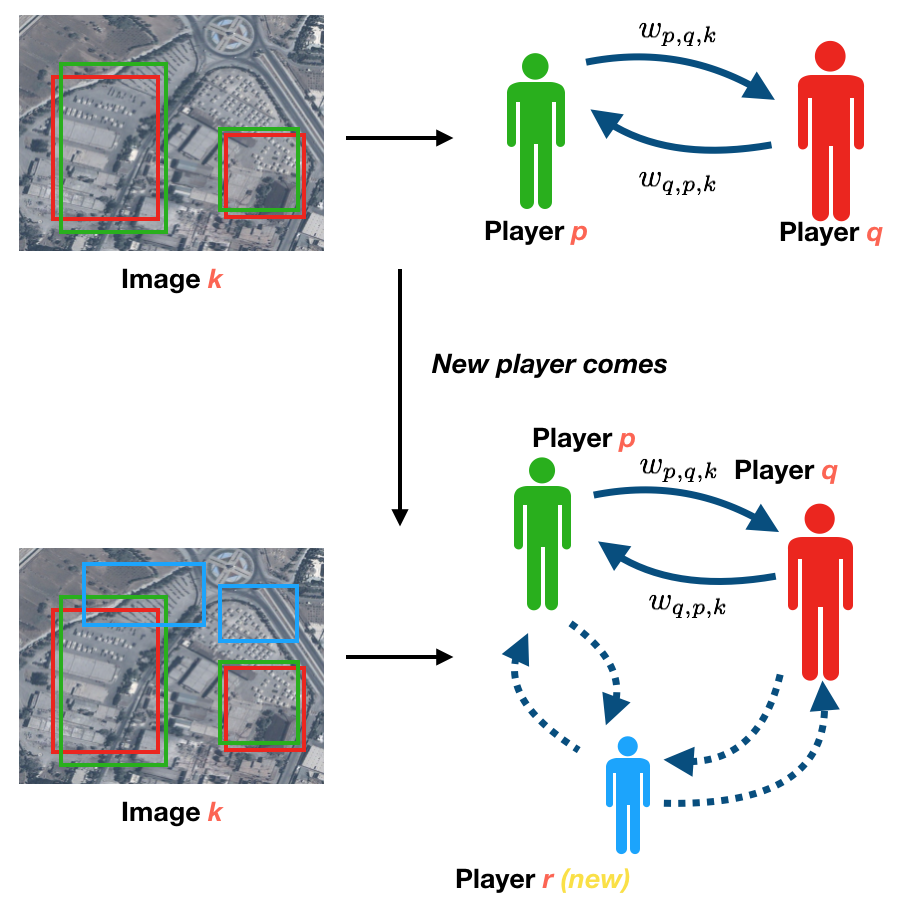
\includegraphics[width=0.5\columnwidth]{figures/graph2}
\caption{Player Rating Graph for Certain Images}
\label{fig:graph}
\end{figure}

\begin{definition}
\label{def:weightv}
\emph{
Assuming the database stores $n$ different tags $\text{tag}_1, \text{tag}_2, ..., \text{tag}_n$ in the system,
The \textbf{System Weight Vector} $v = (p(\text{tag}_1), p(\text{tag}_2), ..., p(\text{tag}_n))$ 
\textbf{of all tags} can be calculated by the following Equation \ref{eq:ptag}:
\begin{equation}
\label{eq:ptag}
p(\text{tag}_i) = \frac{|\text{tag}_i|}{\sum_{j=1}^{n}{|\text{tag}_j|}}
\end{equation}
where  $|\text{tag}_i|$ is the count of $\text{tag}_i$ in the system.
}
\end{definition}
\begin{definition}
\label{def:weightvk}
\emph{
Assuming there are $r_s$ different tags $\text{tag}_{r_1}, \text{tag}_{r_2}, ..., \text{tag}_{r_s}$ were tagged in
a certain image $k$, the \textbf{Image Weight Vector} is a vector for image $k$ that is
composed by part of the System Weight Vector, which 
is donated by $v_k = (p(\text{tag}_{r_1}), p(\text{tag}_{r_2}), ..., p(\text{tag}_{r_s}))$
with $r_i (i=1,2,...,s) \in \{1, 2, ..., n\}$, $r_i \neq r_j (i\neq j, j=1,2,...,s)$ and $s \leq n$.
}
\end{definition}

For instance, the system have 2 different images. The first image is tagged by two players. One is 
$\text{tag}_1, \text{tag}_2, \text{tag}_5$ and another is $\text{tag}_1, \text{tag}_2$;
The second image is tagged by three players, their results are:
$\text{tag}_1, \text{tag}_2, \text{tag}_5$;
$\text{tag}_2, \text{tag}_4, \text{tag}_5$; 
$\text{tag}_3, \text{tag}_4, \text{tag}_5$. 
Thus, the system currently have 5 different tags $\text{tag}_1, \text{tag}_2, \text{tag}_3, \text{tag}_4, \text{tag}_5$.
Each tags ( $\text{tag}_1$ to $\text{tag}_5$) have corresponding counts: $3, 4, 1, 2, 4$; Therefore the
System Weight Vector is $(\frac{3}{14}, \frac{2}{7}, \frac{1}{14}, \frac{1}{7}, \frac{2}{7})$;
the Image Weight Vector of the first image is $(\frac{3}{14}, \frac{2}{7}, \frac{2}{7})$
since the first image only is tagged by $\text{tag}_1, \text{tag}_2, \text{tag}_5$, and
the Image Weight Vector of the second image is as same as the System Weight Vector
due to the second image is tagged by all exist tags.

Obviously, we have $0 \leq p(\text{tag}_i)\leq 1$, $\sum_{i=1}^{n}{p(\text{tag}_{i})}=1$ and $\sum_{i=1}^{s}{p(\text{tag}_{r_i})} \leq 1$.

To go so far as to this system, our player have two different type of inputs: \textbf{the \hyperref[def:roi]{ROI}, 
and its \hyperref[def:tagv]{Tag Vector}}. To define the \hyperref[idx:prg]{PRG} edge weight, 
we introduce two input measurements in the subsequent Definition \ref{def:prmr} and \ref{def:pitc}.

\begin{definition}
\label{def:prmr}
\emph{
The \textbf{Players ROI Matching Ratio (PRMR)} is an importance measurement that measures the proportion of
two different \hyperref[def:roi]{ROI} intersection surface from player $p, q$ and 
the \hyperref[def:roi]{ROI} surface from player $p$ in a certain image $k$, 
which is donated by the following formula:
\begin{equation}
\text{PRMR}(p, q, i, j, k) = \frac{| ROI_{p,i,k} \cap ROI_{q,j,k} | }
       {|ROI_{p,i,k}|}
\end{equation}
where
\begin{itemize}
\item $ROI_{p, i, k}$ is the $i$-th selected ROI from player $p$;
\item $|ROI_{p, i, k}|$ is the surface of $ROI_{p, i, k}$;
\end{itemize}
}
\end{definition}

\begin{lemma}
\label{lemma:prmrrange}
\begin{equation}
\label{eq:prmrrange}
0 \leq \text{PRMR}(p, q, i, j, k) \leq 1
\end{equation}
\end{lemma}
\begin{proof}
According to the Definition of \hyperref[def:roi]{ROI}, $| ROI_{p,i,k} \cap ROI_{q,j,k} |$ 
can archive its maximum value only and only if $ROI_{p,i,k} =  ROI_{q,j,k}$ 
as well as its minimum value only and only if $ROI_{p,i,k}$ has no intersection with $ROI_{q,j,k}$.
Thus:
\[
0 = \frac{0}{|ROI_{p,i,k}|} \leq \text{PRMR}(p, q, i, j, k) \leq
\frac{| ROI_{p,i,k} \cap ROI_{p,i,k} | }{|ROI_{p,i,k}|} = \frac{|ROI_{p,i,k}|}{|ROI_{p,i,k}|} = 1.
\]
\end{proof}

\begin{definition}
\label{def:pitc}
\emph{
The \textbf{Players Input Tag Correlation (PITC)} is an importance measurement that measures the proportion of
the covariance of two different \hyperref[def:tagv]{Tag Vector $T_{p,i,k}, T_{q,j,k}$} from player $p, q$ and the covariance of $T_{p,i,k}$ from player $p$ with itself under the
\hyperref[def:weightvk]{Image Weight Vector $v_k$}, which is donated by the following formula:
\begin{equation}
\text{PITC}(p, q, i, j, k) = \frac{Cov(T_{p,i,k}, T_{q,j,k}; v_k)}{Cov(T_{p,i,k}, T_{p,i,k}; v_k)}
\end{equation}
where $Cov(X, Y; w)$ is the weighted covariance between $X$ and $Y$, which donated by:
\begin{equation}
\label{eq:cov}
Cov(X, Y; w) = \frac{\sum_{i=1}^{n}{w_i(x_i-\frac{1}{n}\sum_{i=1}^{n}{w_i x_i})(y_i-\frac{1}{n}\sum_{i=1}^{n}{w_i y_i})}}{\sum_{i=1}^{n}{w_i}}
\end{equation}
with $X = (x_1, x_2, ..., x_n), Y = (y_1, y_2, ..., y_n), w = (w_1, w_2, ..., w_n)$.
}
\end{definition}

Note that

\begin{enumerate}
\item \textbf{The definition of PRMR and PITC share the same intent for measureing asymmetric importance  
      between player $p$ and player $q$ (how $p$ think of $q$)};
\item The definition of \textbf{PRMR is inspired by} a wide-used computer vision criteria, the so called \textbf{Intersection over Union (IoU)}, 
      also as known as \textbf{Jaccard Index} \cite{real1996probabilistic, jaccard1901etude},
      which is a statistic used for comparing the similarity and diversity of sample sets. 
      However, in our case, we only divided by to guarantee the asymmetric property for directed graph weight;
\item The definition of \textbf{PITC is inspired by the Weighted Pearson Correlation Coefficient} \cite{pearson1895note},
      which is a measure of the linear correlation between two variables. In our case, with the same intent of PRMR, 
      we \textbf{drop} the
      part of covariance of player $q$ in denominator to guarantee the asymmetric property for directed graph weight; 
\item The PRMR and PITC both \textbf{are not metrics} due to $\text{PRMR}(p, q, i, j, k) \neq \text{PRMR}(q, p, i, j, k)$ as well as
$\text{PITC}(p, q, i, j, k) \neq \text{PITC}(q, p, i, j, k)$.
\end{enumerate}

\begin{lemma}
\label{lemma:pitcrange}
\begin{equation}
\label{eq:pitcrange}
-1 \leq \text{PITC}(p, q, i, j, k) \leq 1.
\end{equation}
\end{lemma}
\begin{proof}
We know that the weighted Pearson Correlation Coefficient \cite{pearson1895note} lies on $[-1, 1]$, i.e.
\[
  -1 \leq \frac{Cov(T_{p,i,k}, T_{q,j,k}; v_k)}{\sqrt{Cov(T_{p,i,k}, T_{p,i,k}; v_k)Cov(T_{q,j,k}, T_{q,j,k}; v_k)}} \leq 1
\]
To prove Equation \ref{eq:pitcrange}, we have to show:
\begin{multline}
  \frac{Cov(T_{p,i,k}, T_{q,j,k}; v_k)}{Cov(T_{p,i,k}, T_{p,i,k}; v_k)} \\
  \leq |Cov(T_{q,j,k}, T_{q,j,k}; v_k)\sqrt{Cov(T_{p,i,k}, T_{p,i,k}; v_k)Cov(T_{q,j,k}, T_{q,j,k}; v_k)}| \leq 1
\end{multline}
and
\begin{multline}
  \frac{Cov(T_{p,i,k}, T_{q,j,k}; v_k)}{Cov(T_{p,i,k}, T_{p,i,k}; v_k)} \\
  \geq -|Cov(T_{q,j,k}, T_{q,j,k}; v_k)\sqrt{Cov(T_{p,i,k}, T_{p,i,k}; v_k)Cov(T_{q,j,k}, T_{q,j,k}; v_k)}| \geq -1
\end{multline}
Then we need to show:
\begin{equation}
0 \leq Cov(T_{p,i,k}, T_{p,i,k}; v_k)Cov(T_{q,j,k}, T_{q,j,k}; v_k)^3 \leq 1
\end{equation}
Considering $T_{p,i,k}, T_{q,i,k}$ are described in general, with Equation \ref{eq:cov}, 
we only need to show (\textbf{$s$ is an vector components index} instead of exponential):
\begin{equation}
\label{eq:statement}
0 \leq Cov(T_{p,i,k}, T_{p,i,k}; v_k) = 
\frac{
  \sum_{s=1}^{n}{
    v_{k}^s
    \left(T_{p,i,k}^s - \frac{1}{n}\sum_{s=1}^{n}{v_{k}^s T_{p,i,k}^s}\right)^2
  }
}{
  \sum_{s=1}^{n}{v_{k}^s}
} \leq 1
\end{equation}
According to the definition of \hyperref[def:tagv]{Tag Vector} and \hyperref[def:weightvk]{Image Weight Vector},
the components of $T_{p,i,k}$ are either 1 or 0, 
the components of $v_k$ lies on $[0, 1]$, then we have:
\begin{equation}
0 \leq \left(T_{p,i,k}^s - \frac{1}{n}\sum_{s=1}^{n}{v_{k}^s T_{p,i,k}^s}\right)^2 \leq 1
\end{equation}
Therefore,
\begin{equation}
0 = \frac{
  \sum_{s=1}^{n}{
    v_{k}^s \cdot 0
  }
}{
  \sum_{s=1}^{n}{v_{k}^s}
} 
\leq Cov(T_{p,i,k}, T_{p,i,k}; v_k) \leq
\frac{
  \sum_{s=1}^{n}{
    v_{k}^s \cdot 1
  }
}{
  \sum_{s=1}^{n}{v_{k}^s}
} = 1
\end{equation}
which proves Equation \ref{eq:statement}.
\end{proof}

Thus far, we have enough techniques to define the edge weight of \hyperref[idx:prg]{PRG}.
The definition is shown in Definition \ref{def:edgeweight}.

\begin{definition}
\label{def:edgeweight}
\emph{
For a certain image $k$, the edge weight of the PRG from player $p$ to player $q$ is donated 
by the formula \ref{eq:weight}:
\begin{equation}
\label{eq:weight}
w_{p,q,k} = 
\sum_{j=1}^{n}{
\sum_{i=1}^{m}{ \left(
  \text{PRMR}(p, q, i, j, k)
  \left(
    \text{PITC}(p, q, i, j, k) + 2
  \right)
\right)}}
\end{equation}
with player $p$ selected $m$ ROIs, player $q$ selected $n$ ROIs.
}
\end{definition}

Our goal is to calculate the centrality of the nodes (players) of the network graph.
The \textbf{Perron Frobenius theorem}, proved by Oskar Perron (1907) \cite{perron1907theorie} and Georg Frobenius (1912) \cite{frobenius1912matrizen},
guarantees our goal can be drifted to the calculation of the adjacency matrix of \hyperref[idx:prg]{PRG}.
In consequence, one can use the normalized adjacency matrix through the following formula \ref{eq:normalize}:

\begin{equation}
\label{eq:normalize}
A_k = (a_{p,q,k}) = (\frac{w_{p,q,k}}{\sum_{q}{w_{p,q,k}}})
\end{equation}

where $k$ is the image indicator.

\begin{theorem}
\label{theorem:property}
The normalized adjacency matrix $A_k$ of PRG of a certain image $k$ is irreducible, real, 
non-negative, column-stochastic, and diagonal element being positive.
\end{theorem}

\begin{proof}
\textbf{Irreducibility}: As shown in figure \ref{fig:graph}, for a certain image $k$, 
the \hyperref[idx:prg]{PRG} is strong connected because the
player who selected ROIs in image $k$ has a direct connection to any other player who also selected ROIs in image $k$ 
(the edge weight is well defined according to Equation \ref{eq:weight}).
Thus, since $A_k$ is an normalized strong connected PRG adjacency matrix, which proves $A_k$ is irreducible.

\textbf{Real elements}: With Lemma \ref{lemma:prmrrange} and \ref{lemma:pitcrange}, each part of the Equation \ref{eq:weight} 
are real number. Thus, of course, the matrix $A_k$ elements are calculated by Equation \ref{eq:normalize} that are real elements.

\textbf{Non-negative elements}: With Lemma \ref{lemma:prmrrange} and \ref{lemma:pitcrange}, we have:
\[
w_{p,q,k} = 
\sum_{j=1}^{n}{
\sum_{i=1}^{m}{ \left(
  \text{PRMR}(p, q, i, j, k)
  \left(
    \text{PITC}(p, q, i, j, k) + 2
  \right)
\right)}} 
\geq
\sum_{j=1}^{n}{
\sum_{i=1}^{m}{ \left(
  0 \cdot
  \left(
    -1 + 2
  \right)
\right)}} = 0
\]
that $w_{p,q,k}$ has its minimum value when $\text{PRMR}(p, q, i, j, k) = 0 (for all i=1,...,m; j=1,...,n)$ 
and $\text{PITC}(p, q, i, j, k) = -1 (\text{for all} i=1,...,m; j=1,...,n)$. Meanwhile,

\[
w_{p,q,k} = 
\sum_{j=1}^{n}{
\sum_{i=1}^{m}{ \left(
  \text{PRMR}(p, q, i, j, k)
  \left(
    \text{PITC}(p, q, i, j, k) + 2
  \right)
\right)}} 
\leq 
\sum_{j=1}^{n}{
\sum_{i=1}^{m}{ \left(
  1 \cdot
  \left(
    1 + 2
  \right)
\right)}} = 3mn
\]

that $w_{p,q,k}$ has its maximum value when $\text{PRMR}(p, q, i, j, k) = 1 (\text{for all} i=1,...,m; j=1,...,n)$ 
and $\text{PITC}(p, q, i, j, k) = 1 (\text{for all} i=1,...,m; j=1,...,n)$.
  
\textbf{Positive diagonal elements}: According to Lemma \ref{lemma:pitcrange}, 
the diagonal elements can be formalized by follows:

\begin{equation}
\begin{aligned}
w_{p,p,k} &= 
\sum_{j=1}^{m}{
\sum_{i=1}^{m}{ 
  \left(
    \text{PRMR}(p, p, i, j, k)
    \left(
      \text{PITC}(p, p, i, j, k) + 2
    \right)
  \right)
}} \\
&\geq \sum_{j=1}^{m}{
\sum_{i=1}^{m}{ \left(
  \frac{| ROI_{p,i,k} \cap ROI_{p,j,k} | }{|ROI_{p,i,k}|}
  \left(
    -1 + 2
  \right)
\right)}} \\
&= \sum_{j=1}^{m}{
\sum_{i=1}^{m}{
  \frac{| ROI_{p,i,k} \cap ROI_{p,j,k} | }{|ROI_{p,i,k}|}
}}\\
&= \sum_{i=j}{\frac{| ROI_{p,i,k} \cap ROI_{p,j,k} | }{|ROI_{p,i,k}|}} 
 + \sum_{i\neq j}{\frac{| ROI_{p,i,k} \cap ROI_{p,j,k} | }{|ROI_{p,i,k}|}}\\
&\geq \sum_{i=j}{\frac{| ROI_{p,i,k} \cap ROI_{p,j,k} | }{|ROI_{p,i,k}|}}\\
&= \sum_{i=1}^{m}{\frac{| ROI_{p,i,k} \cap ROI_{p,i,k} | }{|ROI_{p,i,k}|}}\\
&= \sum_{i=1}^{m}{\frac{| ROI_{p,i,k}|}{|ROI_{p,i,k}|}}\\
&= m > 0
\end{aligned}
\end{equation}

\textbf{Column stochastic}: according to the definition of matrix $A$, the sum of the column
elements are:
\begin{equation}
  \sum_{q}{a_{p,q,k}} 
  = \sum_{q}{ \frac{w_{p,q,k}}{ \sum_{q}{w_{p,q,k}} }}
  = \frac{\sum_{q}{w_{p,q,k}}}{\sum_{q}{w_{p,q,k}}} = 1
\end{equation}
\end{proof}

From the proof of property of positive diagonal elements, we see that the number ``2'' is 
a translation that guarantees $\text{PITC}(p, q, i, j, k)$ lies on $[1, 3]$ which helps us
prove this property successfully.

According to \textbf{Perron Frobenius theorem} \cite{perron1907theorie, frobenius1912matrizen} and 
Theorem \ref{theorem:property},
one can infer that there exists an uniqueness eigenvector $V_k = (TV_{1,k}, ..., TV_{n,k})$ of $A_k$,
the so-called Perron vector, with an uniqueness eigenvalue $\rho(A_k)$ is the spectral	radius
of $A_k$, the so-called Perron root, such that:

\[
A_k \cdot V_k = \rho(A_k) \cdot V_k, TV_{i,k} > 0, \sum_{i=1}^{n}{TV_{i,k}} = 1.
\]

Therefore, we define the trust value of a player:

\begin{definition}
\label{def:tv}
\emph{
A \textbf{Trust Value} $TV_{i,k}$ of player $i$ on image $k$ is a score that
equals to the $i$-th component of the Perron vector of the normalized \hyperref[idx:prg]{PRG} adjacency matrix $A_k$.
}
\end{definition}

This definition represents the rating score from player $p$ to player $q$ for a certain image $k$, as same as the centrality
of the player $q$. With the trust value of players, we propose our classification algorithm:

\begin{algorithm}[H]
\label{algo:malicious}
\SetAlgoLined
\SetKwInOut{Input}{input}\SetKwInOut{Output}{output}
\Input{New Player $p$,\\
       Trusted Player $p1, p2, ..., p_m$,\\
       Task Images $k_1, k_2, ..., k_{2n}$,\\
       Acceptance Threshold $\delta$}
\Output{Reliability of Player $p$}
\Begin{
  counter $\longleftarrow$ 0\\
  \For{$k \in [k_1, k_2, ..., k_{2n}]$}{
    \If{$k$ is tagged image}{
      calculate $TV_{p,k}, TV_{p_1,k}, ..., TV_{p_m,k}$\\
      \If{$TV_{p,k} \geq \frac{1}{m}\sum_{i=1}^{m}{TV_{p_i, k}}$}{
        counter $\longleftarrow$ counter $+ 1$
      }
    }
  }
  \eIf{counter $\geq \delta$}{
    reliability $\longleftarrow$ true
  }{
    reliability $\longleftarrow$ false
  }
}
\caption{Malicious Player Detection Algorithm}
\end{algorithm}

The purpose of this algorithm is simple, the criterion of classifying new players performs the action that 
the trust value of a new player should not be less than the mean value of overall trust value of players on image $k$, 
which means the tagging performance of new player should not worth than result performance of former players.
The acceptance threshold is a customizable parameter that can be set by system manager.
For instance, if $\delta = 1$, then the new player only need pass one singular image of all tagged images; 
if $\delta = n$ (half images of the task), then the new player have to pass all tagged images;

Note that sometimes new player carries new tags to the system, this will influence the \hyperref[def:tagv]{Tag Vector} calculation,
which causes the weight are not computable due to 
the dimension of the \hyperref[def:tagv]{Tag Vector} of new player and old player inequal.
We also address a solution for this issue via the following steps:

\begin{itemize}
\item If a new player does not provide new tag: directly perform the calculation with Algorithm \ref{algo:malicious};
\item If a new player carries new tags: Directly drop, it is an unreliable result;
\item If a player carries selected tags and also new tags: 
  \begin{enumerate}
    \item Perform the calculation with Algorithm \ref{algo:malicious} without new tags;
    \item Merge and update all weight vector $v$ via formula \ref{eq:weight} if the player is reliable, 
    \item Otherwise drop and mark the result is unreliable.
  \end{enumerate}
\end{itemize}

\subsubsection{Disaster Evaluation Model}
\label{chapter:dem}

Pooling is an useful technique for training Convolutional Neuron Networks \cite{ciresan2011flexible, krizhevsky2012imagenet},
which combine the outputs of neuron clusters at one layer into a single neuron in the next layer.
It is a kind of aggregation method for an image region.
General pooling techniques are mean pooling, max pooling and stochastic pooling.
The he stochastic pooling uses the weighted average value from 
each of a cluster of neurons at the prior layer \cite{ciregan2012multi}.
We shift this technique to define our Disaster Evaluation Model.

For a monitor region at time $t$, we address the \textbf{\hyperref[idx:dem]{DEM}} 
via disaster level definition as follows:

\begin{definition}
\label{def:dl}
\emph{
Let a monitor region is composed by images $k_1, ..., k_n$, and players $p_1, p_2, ..., p_m$
are tagged these images. The player $p_j$ tagged $r_{j,i}$ ROIs in image $k_i$ with $j=1, ..., m; i=1, ..., n$.
The \textbf{Disaster Level (DL)} of a monitor region is calculated by the following:
\begin{equation}
\label{eq:dl}
DL = v \cdot 
  \left(
    \frac{1}{m}
    \sum_{j=1}^{m}{
      \sum_{i=1}^{n}{
          T_{ p_{j}, r_{j,i}, k_{i} }
      }
    }
  \right)
\end{equation}
with $v$ is the \hyperref[def:weightv]{System Weight Vector} and 
$ T_{ p_{j}, r_{j,i}, k_{i} } $ is the \hyperref[def:tagv]{Tag Vector} of the $r_{j,i}$-th ROI of player $p_j$ in image $k_i$.
}
\end{definition}

With this Definition \ref{def:dl}, we can calculate the disaster level for a monitoring region 
according to Equation \ref{eq:dl} directly.

\subsection{Model Initialization}
\label{chapter:modelinit}

A cold start of such a system is a common problem in human computation system that 
is avoided by hiring people to play or learn as long as 
the number of users or the quantity of data is insufficient.
In this system, we have only have to consider one system initialization issue of cold start.

\begin{figure}[htp]
\centering
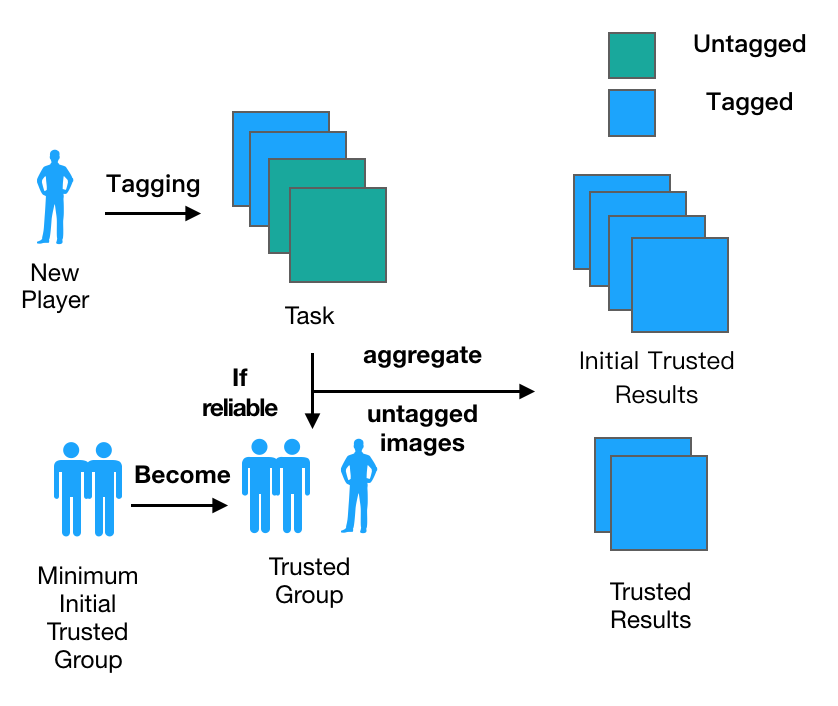
\includegraphics[width=0.5\columnwidth]{figures/coldstart2}
\caption{Initialization of \hyperref[idx:prm]{PRM}}
\label{fig:cold}
\end{figure}

The issue appears in the \hyperref[idx:ptg]{PTG}. 
To initialize the whole system, we need to address an \textbf{initial trusted group} for \hyperref[idx:ptg]{PTG}; 
they shall tagging enough initial trusted result as well as a fixed predefined tag list 
(contains all of the most important tags that organisation need to monitoring)
for \hyperref[idx:ptg]{PTG} and then assign the tagged images to new upcoming players. 
In this system, we do not need to hire people to player and keep the system runs well. This is because: 
when a new player is reliable, then the result of this player will become reliable. 
Meanwhile, the trusted group and available dataset grow larger with this step repeatedly, 
as shown in figure \ref{fig:cold}.

Thus, the final question of our system relate to the minimum number of the initial trusted group.
Our Player Rating Model is based on graph centrality calculation, which means we need a (at least) two dimentional matrix
to perform the overall model calculation. Hence, with the new player, \textbf{the minimum number of the inital trusted group is 1}.
Then the initial trusted group (one person) with the new player composed to a two dimentional adjacency matrix that makes the model
computable.

\subsection{Model Discussion}

TODO: brief disscuss the image independent model is not suitable